\section{Results}

\subsection{Fixed GPS Spoofing}

\begin{figure}[H]
    \centering
    \begin{subfigure}{.5\textwidth}
        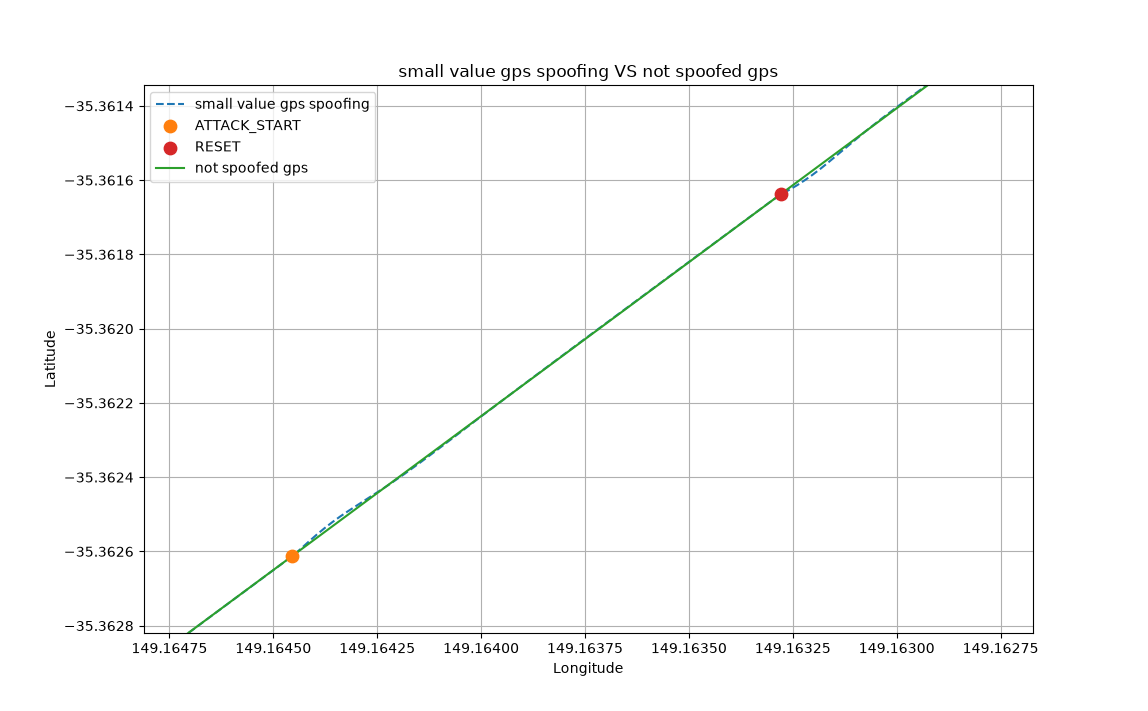
\includegraphics[width=\linewidth]{Data/Images/small_glitch_0.00003/small_gps_spoof.png}
        \caption{Small glitch test.}
        \label{fig:small_glitch_graph}
    \end{subfigure}%
    \begin{subfigure}{.5\textwidth}
        \centering
        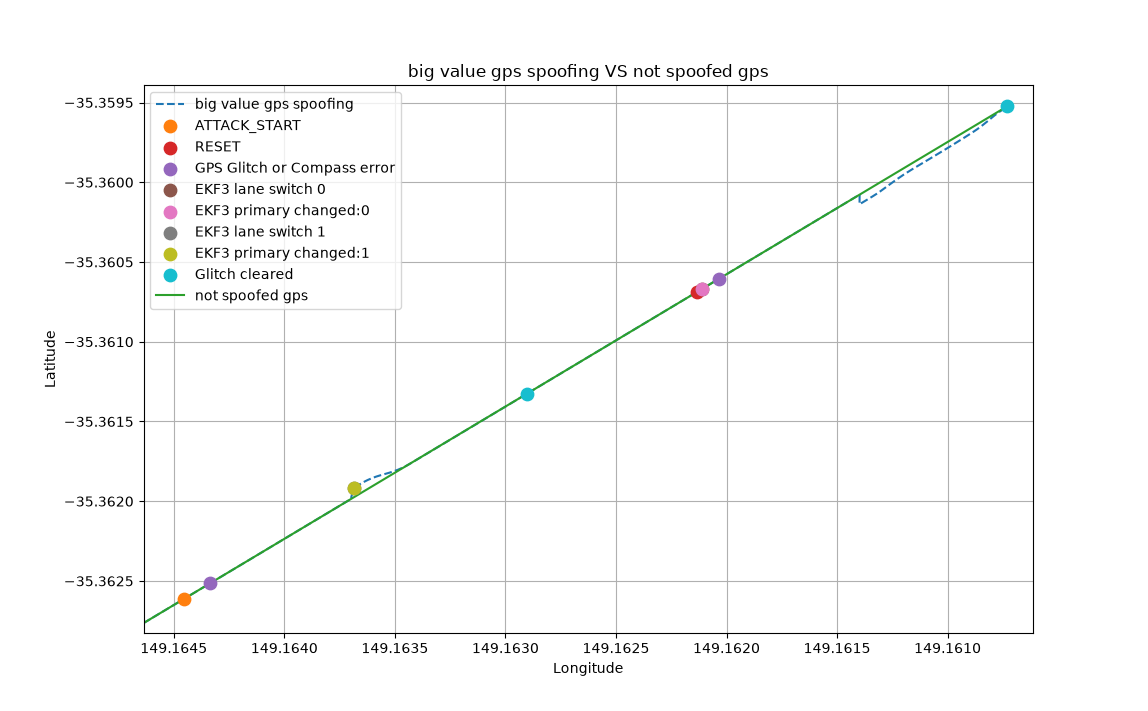
\includegraphics[width=\linewidth]{Data/Images/big_glitch_0.00006/big_gps_spoof.png}
        \caption{Big glitch test.}
        \label{fig:big_glitch_graph}
    \end{subfigure}
    \caption{Graphs of the fluctuations in the GPS position during the fixed GPS spoofing tests.}
\end{figure}

As can be seen in both figures, the introduction of the glitch is clearly visible in the graph, with a sudden jump in the GPS position corresponding to the applied offset. In the case of the small glitch (Figure \ref{fig:small_glitch_graph}), the jump is relatively minor, and the GPS position quickly returns to its original trajectory. In contrast, the big glitch (Figure \ref{fig:big_glitch_graph}) shows a more pronounced jump both when it is introduced and when it is reset, followed by messages stating the detection of a GPS glitch and the subsequent realignment of the GPS position with the estimated vehicle position. Notable is the presence of EKF3 lane switch and EKF3 primary changed events, which indicate a change in the EKF3 estimator configuration as the system compensates for the inconsistent GPS measurements.%and choose a better sensor to rely on. The GPS position eventually realigns with the estimated vehicle position, demonstrating the system's ability to recover from the introduced glitch.

\subsection{Progressive/Adaptive GPS Spoofing}

\begin{figure}[H]
    \centering
    
\includegraphics[width=0.8\linewidth]{progressive_glitch/progressive_gps_spoof.png}
    \caption{Graph of the fluctuations in the GPS position during the progressive GPS spoofing test.}
    \label{fig:progressive_glitch_graph}
\end{figure}

The graph in Figure \ref{fig:progressive_glitch_graph} compares the GPS trajectory obtained during the progressive spoofing test with the trajectory recorded in the absence of spoofing. Throughout most of the experiment, the two trajectories overlap almost completely, indicating that the progressive increase of the applied glitch does not produce a detectable GPS glitch or compass error. The flight controller therefore continues to accept the GPS measurements and the vehicle follows the intended trajectory without triggering the previously observed glitch protection mechanisms.

A significant difference can instead be observed at the end of the experiment, when the applied glitch is reset to zero. This sudden removal of the offset causes an abrupt discontinuity in the spoofed GPS position, visible as the dashed blue segment extending towards the right-hand side of the figure. This segment should be interpreted in the opposite direction, from right to left: the GPS position first jumps away from the previously followed trajectory and then progressively returns towards the final position of the non-spoofed trajectory as the GPS position is realigned with the estimated vehicle position.

This behaviour is consistent with the sudden removal of the accumulated GPS offset. While the progressive spoofing phase allows the GPS position to remain sufficiently close to the position expected by the flight controller, resetting the glitch instantaneously removes the accumulated displacement. The resulting discrepancy is therefore much larger and produces the visible transient realignment at the end of the experiment.